%%%%%   Ingreso General al Sistema para los actores  %%%%%
\chapter{Ingreso al Sistema} \label{chp:IngresoSistema}

	En el presente capítulo se describe el procedimiento general para ingresar al TESSERACT, para lo cual deberá tener a la mano su \textbf{Usuario} y \textbf{Contraseña}, así como la dirección electrónica actual de TESSERACT.

	%Procedimiento
	\subsection{Procedimiento}

		%Pasos de procedimiento
		\begin{enumerate}		
			%Ingresa dirección
			\item Ingrese a la dirección electrónica de TESSERACT desde su navegador.
			%Muestra login
			\item Se mostrará la pantalla \ref{fig:InicioSesion}.
				%Pantalla
				\begin{figure}[htbp!]
					\begin{center}
						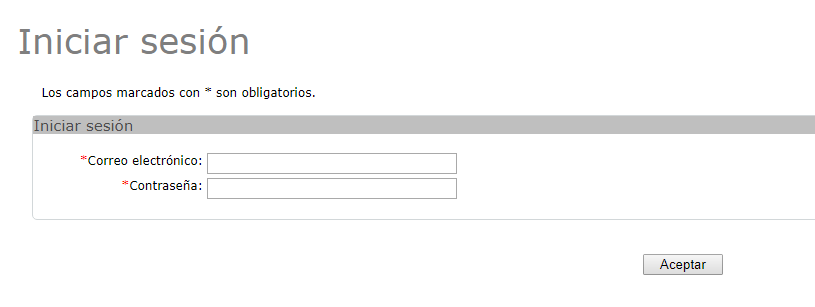
\includegraphics[scale=0.7]{images/inicioSesion/IU1_IniciarSesion}
						\caption{Inicio de Sesión}
						\label{fig:InicioSesion}
					\end{center}
				\end{figure}
			%Ingresa Credenciales
			\item Ingrese su \textbf{Usuario} y \textbf{Contraseña}
			%Aceptar
			\item Presione el botón \IUAceptar.
			%Bienvenida
			\item Se mostrará la pantalla \ref{fig:GPAD} o \ref{fig:GPCOL} dependiendo del rol con el ingresó al sistema.
				%Pantalla
				\begin{figure}[htbp!]
					\begin{center}
						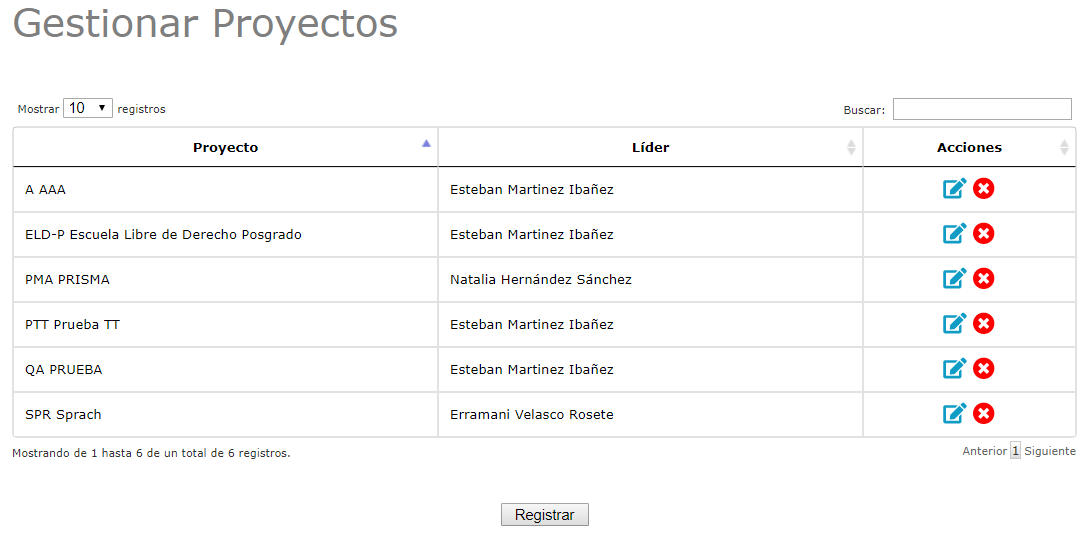
\includegraphics[scale=0.5]{images/inicioSesion/IU2GestionProyectos}
						\caption{Gestionar Proyectos de Administrador}
						\label{fig:GPAD}
					\end{center}
				\end{figure}
			
			\begin{figure}[htbp!]
				\begin{center}
					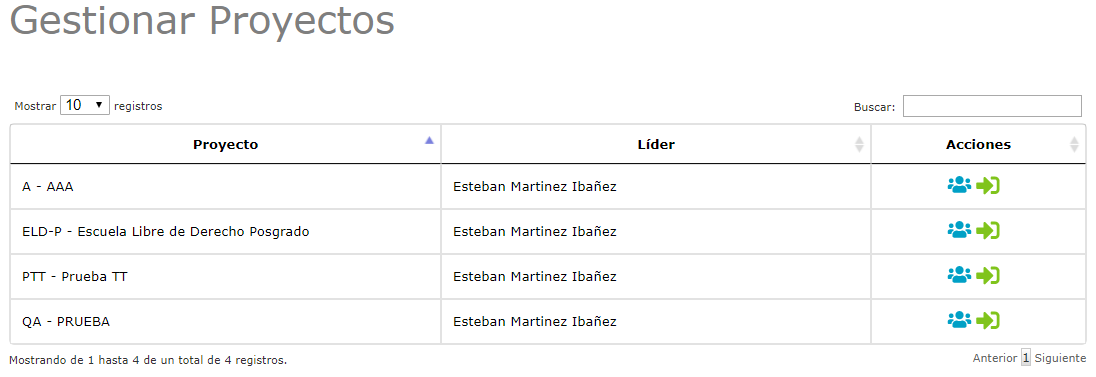
\includegraphics[scale=0.5]{images/inicioSesion/IU5gestionarproyectosColaborador}
					\caption{Gestionar Proyectos de Colaborador}
					\label{fig:GPCOL}
				\end{center}
			\end{figure}

		\end{enumerate}
	PENDIENTE
	%Errores Comunes
	\begin{Errores}
		
		%Template de \error
		%\error{El sistema muestra un mensaje que indica que la información ingresada en un campo no tiene el formato correcto.}{
		%	\begin{itemize}
		%		\UCli Verifique que haya ingresado la información en cada uno de los campos marcados con un *.
		%	\end{UClist}
		%}
		%Campos obligatorios
		\error{El sistema muestra un mensaje que indica que un campo obligatorios estan siendo omitido.}{
			Verifique que haya ingresado información en cada uno de los campos marcados con un *
		}
		%Formato correcto
		\error{El sistema muestra un mensaje que indica que la información ingresada en un campo no tiene el formato correcto.}{Verifique que haya ingresado la información en cada uno de los campos marcados con un *.
		}
		%Longitud
		\error{El sistema muestra un mensaje que indica que alguno o todos los campos obligatorios estan siendo omitidos.}{Verifique que haya ingresado información en cada uno de los campos marcados con un *.
		}
		
	\end{Errores}
	
	%Características de los Campos de entrada
	\begin{Campos}
		
		%Características: Nombre
		\campo{Usuario}{Letras}{máximo 50 caracteres}{administrador}
		%Características: Contraseña
		\campo{Contraseña}{Letras}{máximo 50 caracteres}{+d4v1d}		
	\end{Campos}